\documentclass[a4paper]{article}

\usepackage[utf8]{inputenc}
\usepackage[T1]{fontenc}
\usepackage[spanish]{babel}
\usepackage[margin={20mm,25mm}]{geometry}

\usepackage{ifthen}
\usepackage{mathtools}
\usepackage{xcolor}
\usepackage{booktabs}
\usepackage{circuitikz}
\usepackage{fancyhdr}
\usepackage{parskip}
\usepackage{hyperref}
\usepackage{graphicx}
\usepackage{tikz}
\usetikzlibrary{karnaugh,arrows,automata}
\tikzset{
    %Define standard arrow tip
    >=stealth',
    % Define arrow style
    pil/.style={
           ->,
           thick,}
}
\def\checkmark{\tikz\fill[scale=0.4](0,.35) -- (.25,0) -- (1,.7) -- (.25,.15) -- cycle;}

% --------------------
% DATOS DEL INFORME
\newcommand{\numeroTarea}   {1}                 % <-- Reemplazar X con el número de la tarea
\newcommand{\numeroGrupo}   {29}                 % <-- Reemplazar N con el número de su grupo
\newcommand{\nombrePrimero} {Diego Paz}    % <-- Reemplazar con el nombre del primer integrante
\newcommand{\rolPrimero}    {202004502-k}        % <-- Reemplazar con el rol del primer integrante
\newcommand{\nombreSegundo} {Ronald Bruno}    % <-- Reemplazar con el nombre del segundo integrante
\newcommand{\rolSegundo}    {202030563-3}        % <-- Reemplazar con el rol del segundo integrante
% --------------------

% --------------------
% NO MODIFICAR ESTA PARTE
\title{Informe Tarea \numeroTarea \\ \large
    \ifthenelse{\equal{\numeroTarea}{1}}{Circuito Combinacional}{}
    \ifthenelse{\equal{\numeroTarea}{2}}{Circuito Secuencial}{}
    \ifthenelse{\equal{\numeroTarea}{3}}{Lenguajes de Descripción de Hardware}{}
    \ifthenelse{\equal{\numeroTarea}{4}}{ARM Assembly}{}
    \ifthenelse{\equal{\numeroTarea}{X}}{Tema de la tarea}{}
}
\author{\textbf{Grupo \numeroGrupo} \\ \begin{tabular}{r @{\quad} l}
    \nombrePrimero & \rolPrimero \\
    \nombreSegundo & \rolSegundo
\end{tabular}}
\date{\today}

\setlength{\parindent}{15pt}
\addto\captionsspanish{\renewcommand{\tablename}{Tabla}}
% --------------------

\begin{document}

\begin{titlepage}
    \maketitle
    \thispagestyle{empty}
    
    \begin{abstract}
        En este informe abarcamos el desarrollo de un circuito que se nos pide que cumpla con ciertas condiciones y prioridades, en este caso, un robot que debe moverse según su nivel de batería y de la cantidad de enemigos y cargas que tenga en las celdas adyacentes a sí mismo. Mediante tablas de verdad y mapas de Karnaugh se logró llegar a un circuito que cumple con todos los requisitos descritos en el enunciado de la tarea y pasó los casos de prueba aplicados. Se aplicó conceptos y herramientas tales como el selector de Bits para poder simplificar una entrada de 4 bits a una de 1 bit, se agrupó correctamente los minterminos de los mapas de Karnaugh para expresar correctamente las ecuaciones booleanas de cada una de las salidas y se logró simplificar un circuito de 10 bits de entrada totales a uno de 7 bits, para luego ingresar las ecuaciones booleanas obtenidas al software de modelacion de circuitos digitales $Logisim$ y comprobar nuestros resultados obtenidos y dar una solución concreta a la problematica planteada en el ejercicio.
    \end{abstract}
    
    \vfill
    \tableofcontents
\end{titlepage}

\section{Desarrollo de la tarea}

En el enunciado se nos presenta un modelo conceptual de robot cuya funcionalidad es elegir entre 3 celdas para moverse dependiendo si hay enemigos o cargas en estas, y si el robot está por sobre un umbral de carga en su batería, estas condiciones están representadas en el caso de la batería por 1 pin de 4 bits, y tanto los enemigos como las cargas estan representados por 3 pines de 1 bit, y el circuito en su totalidad debe entregar 3 salidas de 1 bit, dependiendo de hacia donde debe moverse el robot.
Además, se nos encarga modelar este robot y construir su circuito correspondiente en \textit{Logisim}, y para esto primero se debe analizar el enunciado.

Se nos dice que la batería del robot está representada por un pin de 4 bits, y que el comportamiento del robot cambia dependiendo si esta entrada de 4 bits tiene un valor menor o igual que 3, por lo que si el pin tiene alguno de los siguientes valores, el comportamiento del robot cambia: \{0000, 0001, 0010, 0011\}. Viendo esto, podemos notar que se mantienen constantes los valores de los bits 3 y 2, entonces utilizando un selector de bits en Logisim, podemos transformar esta entrada de 4 bits en una de 1 bit, que llamaremos $B$, donde será 1 si la entrada es menor que 4, y 0 para valores iguales o mayores que 4, tal como se muestra en la siguiente tabla:

\begin{table}[!htbp]
    \centering
    \begin{tabular}{cccc|c}
    $B_3$ & $B_2$ & $B_1$ & $B_0$ & $B$ \\ \hline
    0     & 0     & 0     & 0     & 1   \\
    0     & 0     & 0     & 1     & 1   \\
    0     & 0     & 1     & 0     & 1   \\
    0     & 0     & 1     & 1     & 1   \\
    0     & 1     & 0     & 0     & 0   \\
    0     & 1     & 0     & 1     & 0   \\
    0     & 1     & 1     & 0     & 0   \\
    0     & 1     & 1     & 1     & 0   \\
    1     & 0     & 0     & 0     & 0   \\
    1     & 0     & 0     & 1     & 0   \\
    1     & 0     & 1     & 0     & 0   \\
    1     & 0     & 1     & 1     & 0   \\
    1     & 1     & 0     & 0     & 0   \\
    1     & 1     & 0     & 1     & 0   \\
    1     & 1     & 1     & 0     & 0   \\
    1     & 1     & 1     & 1     & 0  
    \end{tabular}
    \caption{Tabla de verdad del comportamiento de la batería.}
    \label{tab1}
\end{table}

Una vez simplificado la primera entrada, es necesario trabajar las otras 6, pero una tabla de verdad de 6 variables sería muy grande al tener 128 filas, entonces utilizaremos mapas de Karnaugh, donde utilizaremos 2 mapas (para cuando el valor de la batería es 0 o 1) por cada salida (L, F, R), ya que además pueden mostrar la representacion con minterminos de la ecuación booleana del circuito.
\newpage
Entonces, para la salida \textbf{\textit{L}}, cuando $B = 0$, el mapa de Karnaugh es:

\begin{tikzpicture}[karnaugh, American style,
                    thick,
                    grp/.style n args={3}{#1,fill=#1!30,
                    minimum width=#2\kmunitlength,
                    minimum height=#3\kmunitlength,
                    rounded corners=0.2\kmunitlength,
                    fill opacity=0.6,
                    rectangle,draw}]
    \karnaughmap{6}{$L(E_L,E_F,E_R,C_L,C_F,C_R)$}{{$E_L$}{$E_F$}{$E_R$}{$C_L$}{$C_F$}{$C_R$}}%
        {0000000000000000111111111111111100000000000000000000000000000000}
        {
            \node[grp={blue}{3.8}{3.8}](n000) at (6.0,6.0) {};
        }
    
\end{tikzpicture}

Y cuando $B = 1$, el mapa de Karnaugh es:

\begin{tikzpicture}[karnaugh, American style,
                    thick,
                    grp/.style n args={3}{#1,fill=#1!30,
                    minimum width=#2\kmunitlength,
                    minimum height=#3\kmunitlength,
                    rounded corners=0.2\kmunitlength,
                    fill opacity=0.6,
                    rectangle,draw}]
    \karnaughmap{6}{$L(E_L,E_F,E_R,C_L,C_F,C_R)$}{{$E_L$}{$E_F$}{$E_R$}{$C_L$}{$C_F$}{$C_R$}}%
        {0000100000001100000010100000111100000000000000000000000000000000}
        {
            \node[grp={blue}{3.8}{0.8}](n000) at (4.0,4.5) {};
            \node[grp={orange}{1.8}{1.8}](n001) at (5.0,5.0) {};
            \node[grp={teal}{0.8}{3.8}](n002) at (4.5,6.0) {};
            \node[grp={red}{1.8}{0.8}](n003) at (4.0,7.5) {};
            \node[grp={red}{1.8}{0.8}](n004) at (4.0,4.5) {};
            \draw[red] (n003.west) to [bend right=25] (n004.west)
                       (n003.east) to [bend left=25] (n004.east);
        }
    
\end{tikzpicture}
\vspace{1cm}

Por lo que para este grupo de mapas tenemos que:
\begin{equation}
    B = 0\ ;\  L(E_L,E_F,E_R,C_L,C_F,C_R) = E_F \overline{E_L}
\end{equation}
\begin{equation}
    B = 1\ ;\  L(E_L,E_F,E_R,C_L,C_F,C_R) =  C_L \overline{E_L} E_R \overline{C_F} + C_L \overline{C_R} \overline{E_L} \overline{C_F} + E_F C_L \overline{C_R} \overline{E_L} + E_F C_L \overline{E_L} E_R
\end{equation}
Entoces, al tener B constante en cada mapas, lo agregamos a la expresión, pero antes, podemos ver que en el mapa con B = 1, las expresiones $E_F C_L \overline{C_R} \overline{E_L}$ y $E_F C_L \overline{E_L} E_R$ también se puede agrupar en B = 0, así que como B no sería constante, no se le agrega a estas expresiones, quedando la expresión final para $L$ como:
\begin{equation}
    L(B,E_L,E_F,E_R,C_L,C_F,C_R) = \overline{B} E_F \overline{E_L} + B C_L \overline{E_L} E_R \overline{C_F} + B C_L \overline{C_R} \overline{E_L} \overline{C_F} + E_F C_L \overline{C_R} \overline{E_L} + E_F C_L \overline{E_L} E_R
\end{equation}

\newpage
Para la salida \textbf{\textit{F}}, cuando $B = 0$, el mapa de Karnaugh es:

\begin{tikzpicture}[karnaugh, American style,
                    thick,
                    grp/.style n args={3}{#1,fill=#1!30,
                    minimum width=#2\kmunitlength,
                    minimum height=#3\kmunitlength,
                    rounded corners=0.2\kmunitlength,
                    fill opacity=0.6,
                    rectangle,draw}]
    \karnaughmap{6}{$F(E_L,E_F,E_R,C_L,C_F,C_R)$}{{$E_L$}{$E_F$}{$E_R$}{$C_L$}{$C_F$}{$C_R$}}%
        {1111111111111111000000000000000011111111111111110000000000000000}
        {
            \node[grp={blue}{3.8}{3.8}](n000) at (2.0,2.0) {};
            \node[grp={blue}{3.8}{3.8}](n001) at (2.0,6.0) {};
            \draw[blue] (n000.west) to [bend left=25] (n001.west)
                       (n000.east) to [bend right=25] (n001.east);
        }
    
\end{tikzpicture}

Y cuando $B = 1$, el mapa de Karnaugh es:

\begin{tikzpicture}[karnaugh, American style,
                    thick,
                    grp/.style n args={3}{#1,fill=#1!30,
                    minimum width=#2\kmunitlength,
                    minimum height=#3\kmunitlength,
                    rounded corners=0.2\kmunitlength,
                    fill opacity=0.6,
                    rectangle,draw}]
    \karnaughmap{6}{$F(E_L,E_F,E_R,C_L,C_F,C_R)$}{{$E_L$}{$E_F$}{$E_R$}{$C_L$}{$C_F$}{$C_R$}}%
        {0011001100110011000000000000000000110011001100110000000000000000}
        {
            \node[grp={blue}{3.8}{1.8}](n000) at (2.0,6.0) {};
            \node[grp={blue}{3.8}{1.8}](n001) at (2.0,2.0) {};
            \draw[blue] (n000.west) to [bend right=25] (n001.west)
                       (n000.east) to [bend left=25] (n001.east);
        }
    
\end{tikzpicture}
\vspace{1cm}

Por lo que para este grupo de mapas tenemos que:
\begin{equation}
    B = 0\ ;\  F(E_L,E_F,E_R,C_L,C_F,C_R) = \overline{E_F}
\end{equation}
\begin{equation}
    B = 1\ ;\  F(E_L,E_F,E_R,C_L,C_F,C_R) =  \overline{E_F} C_F
\end{equation}

Entoces, al tener B constante en cada mapas, lo agregamos a la expresión, pero antes, podemos ver que en el mapa con B = 1, la expresión también se puede agrupar en B = 0, así que como B no sería constante, no se le agrega a la expresión, quedando la expresión final para $F$ como:
\begin{equation}
    F(B,E_L,E_F,E_R,C_L,C_F,C_R) = \overline{B} \overline{E_F} + \overline{E_F} C_F
\end{equation}

\newpage
Y para la salida \textbf{\textit{R}}, cuando $B = 0$, el mapa de Karnaugh es:

\begin{tikzpicture}[karnaugh, American style,
                    thick,
                    grp/.style n args={3}{#1,fill=#1!30,
                    minimum width=#2\kmunitlength,
                    minimum height=#3\kmunitlength,
                    rounded corners=0.2\kmunitlength,
                    fill opacity=0.6,
                    rectangle,draw}]
    \karnaughmap{6}{$R(E_L,E_F,E_R,C_L,C_F,C_R)$}{{$E_L$}{$E_F$}{$E_R$}{$C_L$}{$C_F$}{$C_R$}}%
        {0000000000000000000000000000000000000000000000001111111100000000}
        {
            \node[grp={blue}{3.8}{1.8}](n000) at (6.0,1.0) {};
        }
    
\end{tikzpicture}

Y cuando $B = 1$, el mapa de Karnaugh es:

\begin{tikzpicture}[karnaugh, American style,
                    thick,
                    grp/.style n args={3}{#1,fill=#1!30,
                    minimum width=#2\kmunitlength,
                    minimum height=#3\kmunitlength,
                    rounded corners=0.2\kmunitlength,
                    fill opacity=0.6,
                    rectangle,draw}]
    \karnaughmap{6}{$R(E_L,E_F,E_R,C_L,C_F,C_R)$}{{$E_L$}{$E_F$}{$E_R$}{$C_L$}{$C_F$}{$C_R$}}%
        {0100010000000000010101010000000001000100000000000101010100000000}
        {
            \node[grp={blue}{1.8}{1.8}](n002) at (6.0,1.0) {};
            \node[grp={blue}{1.8}{1.8}](n003) at (6.0,7.0) {};
            \node[grp={red}{1.8}{0.8}](n000) at (2.0,7.5) {};
            \node[grp={red}{1.8}{0.8}](n001) at (6.0,7.5) {};
            \node[grp={red}{1.8}{0.8}](n004) at (2.0,0.5) {};
            \node[grp={red}{1.8}{0.8}](n005) at (6.0,0.5) {};
            \draw[red] (n000.north) to [bend left=25] (n001.north)
                       (n001.south) to [bend left=25] (n005.north);
            \draw[red] (n004.north) to [bend left=25] (n000.south)
                        (n004.south) to [bend right=25] (n005.south);
            \draw[blue] (n002.west) to [bend left=25] (n003.west)
                        (n002.east) to [bend right=25] (n003.east);
        }
    
\end{tikzpicture}
\vspace{1cm}

Por lo que para este grupo de mapas tenemos que:
\begin{equation}
    B = 0\ ;\  R(E_L,E_F,E_R,C_L,C_F,C_R) = E_F E_L \overline{E_R}
\end{equation}
\begin{equation}
    B = 1\ ;\  R(E_L,E_F,E_R,C_L,C_F,C_R) =  C_R \overline{E_R} \overline{C_F} + E_F C_R \overline{E_R}
\end{equation}
Entoces, al tener B constante en cada mapas, lo agregamos a la expresión, además, revisamos que ninguna de las expresiones se puede agrupar en el mapa contrario, así quedando la expresión final para $R$ como:
\begin{equation}
    R(B,E_L,E_F,E_R,C_L,C_F,C_R) = \overline{B} E_F E_L \overline{E_R} + B C_R \overline{E_R} \overline{C_F} + B E_F C_R \overline{E_R}
\end{equation}
\newpage
\section{Resultados y análisis}

Una vez terminado el circuito, lo ingresamos a $Logisim$ para ver su comportamiento en casos de prueba.

A continuación se mostraran los circuitos de cada salida por separado y el circuito final.

\begin{figure}[!htbp]
    \centering
    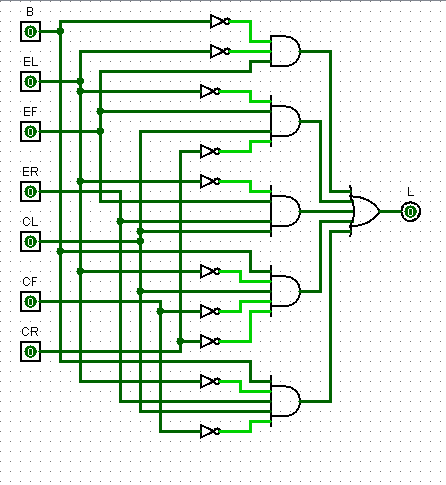
\includegraphics[width=0.6\textwidth]{circuito_L.png}
    \caption{Circuito combinacional de la salida L}
    \label{fig:CircL}
\end{figure}

\begin{figure}[!htbp]
    \centering
    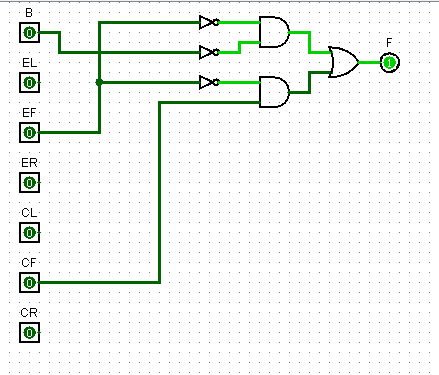
\includegraphics[width=0.6\textwidth]{circuito_F.png}
    \caption{Circuito combinacional de la salida F}
    \label{fig:CircF}
\end{figure}

\begin{figure}[!htbp]
    \centering
    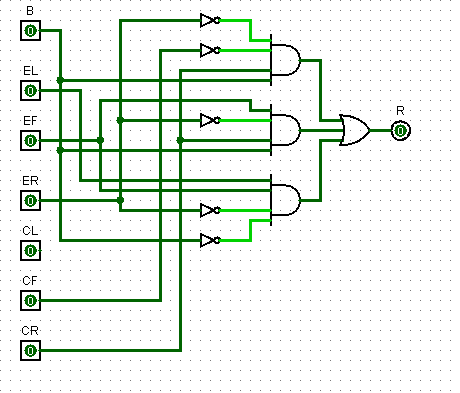
\includegraphics[width=0.6\textwidth]{circuito_R.png}
    \caption{Circuito combinacional de la salida R}
    \label{fig:CircR}
\end{figure}

\begin{figure}[!htbp]
    \centering
    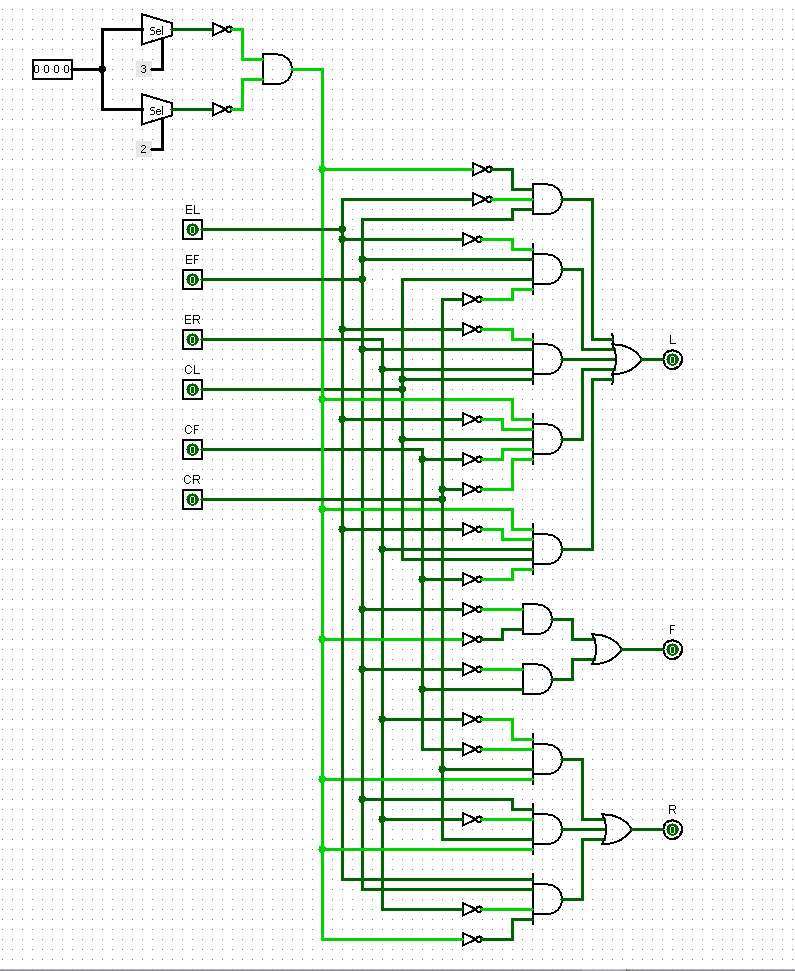
\includegraphics[width=0.6\textwidth]{circuito_final.png}
    \caption{Circuito combinacional final}
    \label{fig:CircFinal}
\end{figure}

alo

\section{Conclusiones}
%{\color{red} Por último acá deben escribir una conclusión respecto a la finalización de la tarea y el nivel de completitud que alcanzaron, en caso de no terminarla. Deben también incluir una reflexión personal respecto a la tarea, los problemas que tuvieron, y qué podrían mejorar en caso de tener que trabajar nuevamente con el contenido de la tarea.}
Hemos creado un circuito combinacional con el objetivo de orientar a nuestro robot en una serie de decisiones, como las de enfrentarse a un oponente, recargar su enregia, o seguir por un camino vacio. Todo esto se resuelve gracias a las tablas de verdad y el mapa de Karnaugh. (... explicar aqui un poco de desarrollo).\\
Finalmente tenemos que nuestro circuito esta totalmente finalizado ya que el robot puede seguir las rutas según el nivel de priorización que se solicitaba.

\end{document}